\chapter{Introduction}
\label{ch:intro}
\chaptermark{Introduction}

%\setcounter{equation}{0}
% ==========================================================================================================
\newpage

The mind-wandering state is a common human experience. Human cognition has the capacity to generate thoughts that are only loosely related to the current external stimulus or any task being performed. However, the content, form, and consequences of the experience that emerge during the mind-wandering state is not well understood (Mittner, Hawkins, Boekel, \& Forstmann, 2016; Seli, Risko, Smilek, \& Schacter, 2016; Smallwood \& Andrews-Hanna, 2013). The current aim is to gain a better understanding of the neuropsychological mechanism of the mind-wandering state.

% ==========================================================================================================

\section{Mind wandering as a Heterogeneous phenomenon}

\subsection{Heterogeneity in definitions}

\subsection{Heterogeneity in functional outcomes}

\subsection{Heterogeneity in experiential profiles }

% ==========================================================================================================

\section{Accounts of Mind Wandering}

\subsection{Representational account}

\subsection{Executive failure account}
Studies have shown that the mind wandering state has different types of content in, such as different time periods, interpersonal relationship, and can be in a deliberate or spontaneous way. The content of spontaneous thoughts can be future- or past-focused (Baird, Smallwood, \& Schooler, 2011; Smallwood \& O’Connor, 2011). Interpersonal social problem solving happens during mind wandering, but the effectiveness of solutions depends on the executive control ability (Ruby, Smallwood, Sackur, \& Singer, 2013). Mind-wandering also reveals the capability of reflecting on the individual’s own thought, known as meta-awareness (Schooler et al., 2011). Deliberate or a spontaneous mind-wandering states influence the traits of the thought contents (Seli, Carriere, \& Smilek, 2014). Studies have shown that there are both costs and benefits associated with mind-wandering. The positive outcomes associated with mind-wandering include increasing creative problem solving (Baird et al., 2011) and create concrete personal goals (Medea et al., 2016). Other research demonstrates that mind-wandering can facilitate recovery from negative affect \cite{Ruby2013a} and provide relief from loneliness (Poerio, Totterdell, Emerson, \& Miles, 2016). It can also lead to negative outcomes, such as depression (Killingsworth \& Gilbert, 2010; Smallwood, O’Connor, Sudbery, \& Obonsawin, 2007) and poor executive control (McVay \& Kane, 2009). These functional outcomes all derive from the mind-wandering state and demonstrate the heterogeneity of mind-wandering. However, we still knows very little about how the various kind of spontaneous thoughts converged as one state that disassociate from the external world. We would like to further examine the common narrative of the heterogeneity of mind-wandering.  
Mind-wandering has the characteristic of both state and a trait. The individual generates different spontaneous thought under different circumstances. Previous studies suggested that under some conditions, people’s mind are more likely to wander. When the mood is negative, the individual is more likely to reduce their attention and is prone to the mind-wandering state (Smallwood, Fitzgerald, Miles, \& Phillips, 2009; Smallwood \& O’Connor, 2011). A non-demanding external situation can lead the disinterested individual to prospect, while in a situation where requires them to focus, there are no difference between future- or past-related thought (Smallwood, Nind, \& O’Connor, 2009). Some psychological mental conditions are indicators of an individual’s tendency to mind-wander.  Studies have shown that personal traits, such as depression and mindfulness, influence the content of spontaneous thought. The depressed individual are more likely to mind-wander and shows a poor performance on the external task (Smallwood et al., 2007). Mindfulness, on the other hand, increases task performance and reduces mind-wandering (Mrazek, Smallwood, \& Schooler, 2012). The mind-wandering state is consistent within certain situations or personal traits. We are interested in finding a common ground to describe these trait- and state-like features of mind-wandering.
% ==========================================================================================================
\section{Neural hierarchies}
\label{intro:neural}

\subsection{Historical perspective}

\subsection{Principle gradient}

\subsection{Multiple demand network }

The recent interesting in the neural basis of the mind-wandering state has revealed the relation between the neural activity during resting state and the heterogeneity of the mind-wandering experience. Evidence from meta-analysis have shown that that task-unrelated thoughts are associated with activity in regions of medial prefrontal cortex, posterior cingulate cortex and in lateral parietal cortex (see Fox, Spreng, Ellamil, Andrews-Hanna, \& Christoff, 2015; Stawarczyk \& D’Argembeau, 2015) - regions that make up the Default Mode Network (DMN; Buckner, Andrews-Hanna, \& Schacter, 2008). One of the well documented functional outcome of the mind-wandering state is poor executive control (McVay \& Kane, 2009), which implies a lack of engagement in the on-going task; therefore DMN and resting state are the interests of the spontaneous thoughts researches. Recent studies have demonstrated the spontaneous thought is related to the changes distributing across a wide range of cortical areas during the resting state   (Gorgolewski et al., 2014)., and the posterior core of DMN act as a hub for information integration (Smallwood et al., 2016). 

Studies on the interactions between other brain regions and the DMN has further proven the integrative nature of the DMN, and the related cognitive processes are also found in the behavioural researches of the mind-wandering state. These evidences support the component processing approach (Smallwood, Gorgolewski, et al., 2013; Smallwood, Ruby, \& Singer, 2013), suggesting that the complexity of the mind-wandering state is related to the combination of multiple subprocess. The interaction between the hippocampus and the DMN is found to serves as the neural basis of mental time travel (Karapanagiotidis, Bernhardt, Jefferies, \& Smallwood, 2017) and goal orientated thoughts (Medea et al., 2016), which support with the behavioural finding of the temporal mind-wandering contents and the involvement of episodic memory.  Study showed that the functional connectivity and cortical thickness of the frontal-parietal network and DMN is related to the spontaneous or deliberate nature of the mind-wandering thought contents (Golchert et al., 2017). The study on the functional gradient organization of cortex indicated that the DMN is the top of the hierarchy of cognition-related processes that integrate trans-modal information (Margulies et al., 2016). Recent study has demonstrated the complex contribution of the DMN to cognition by showing that the functional outcomes of the mind-wandering state are related to specific type of DMN activation and thought content phenotype in multivariate pattern analysis (Wang et al., 2017, under review).  These researches suggested the mind-wandering state and its main neural basis, the DMN, are working in an integrative manner in human cognition. We are interested in further decoding the behavioural and neural features of the mind-wandering state. 
% ==========================================================================================================
\section{Set of considerations for better accounts of cognition}


\begin{figure}[H]
	\centering
	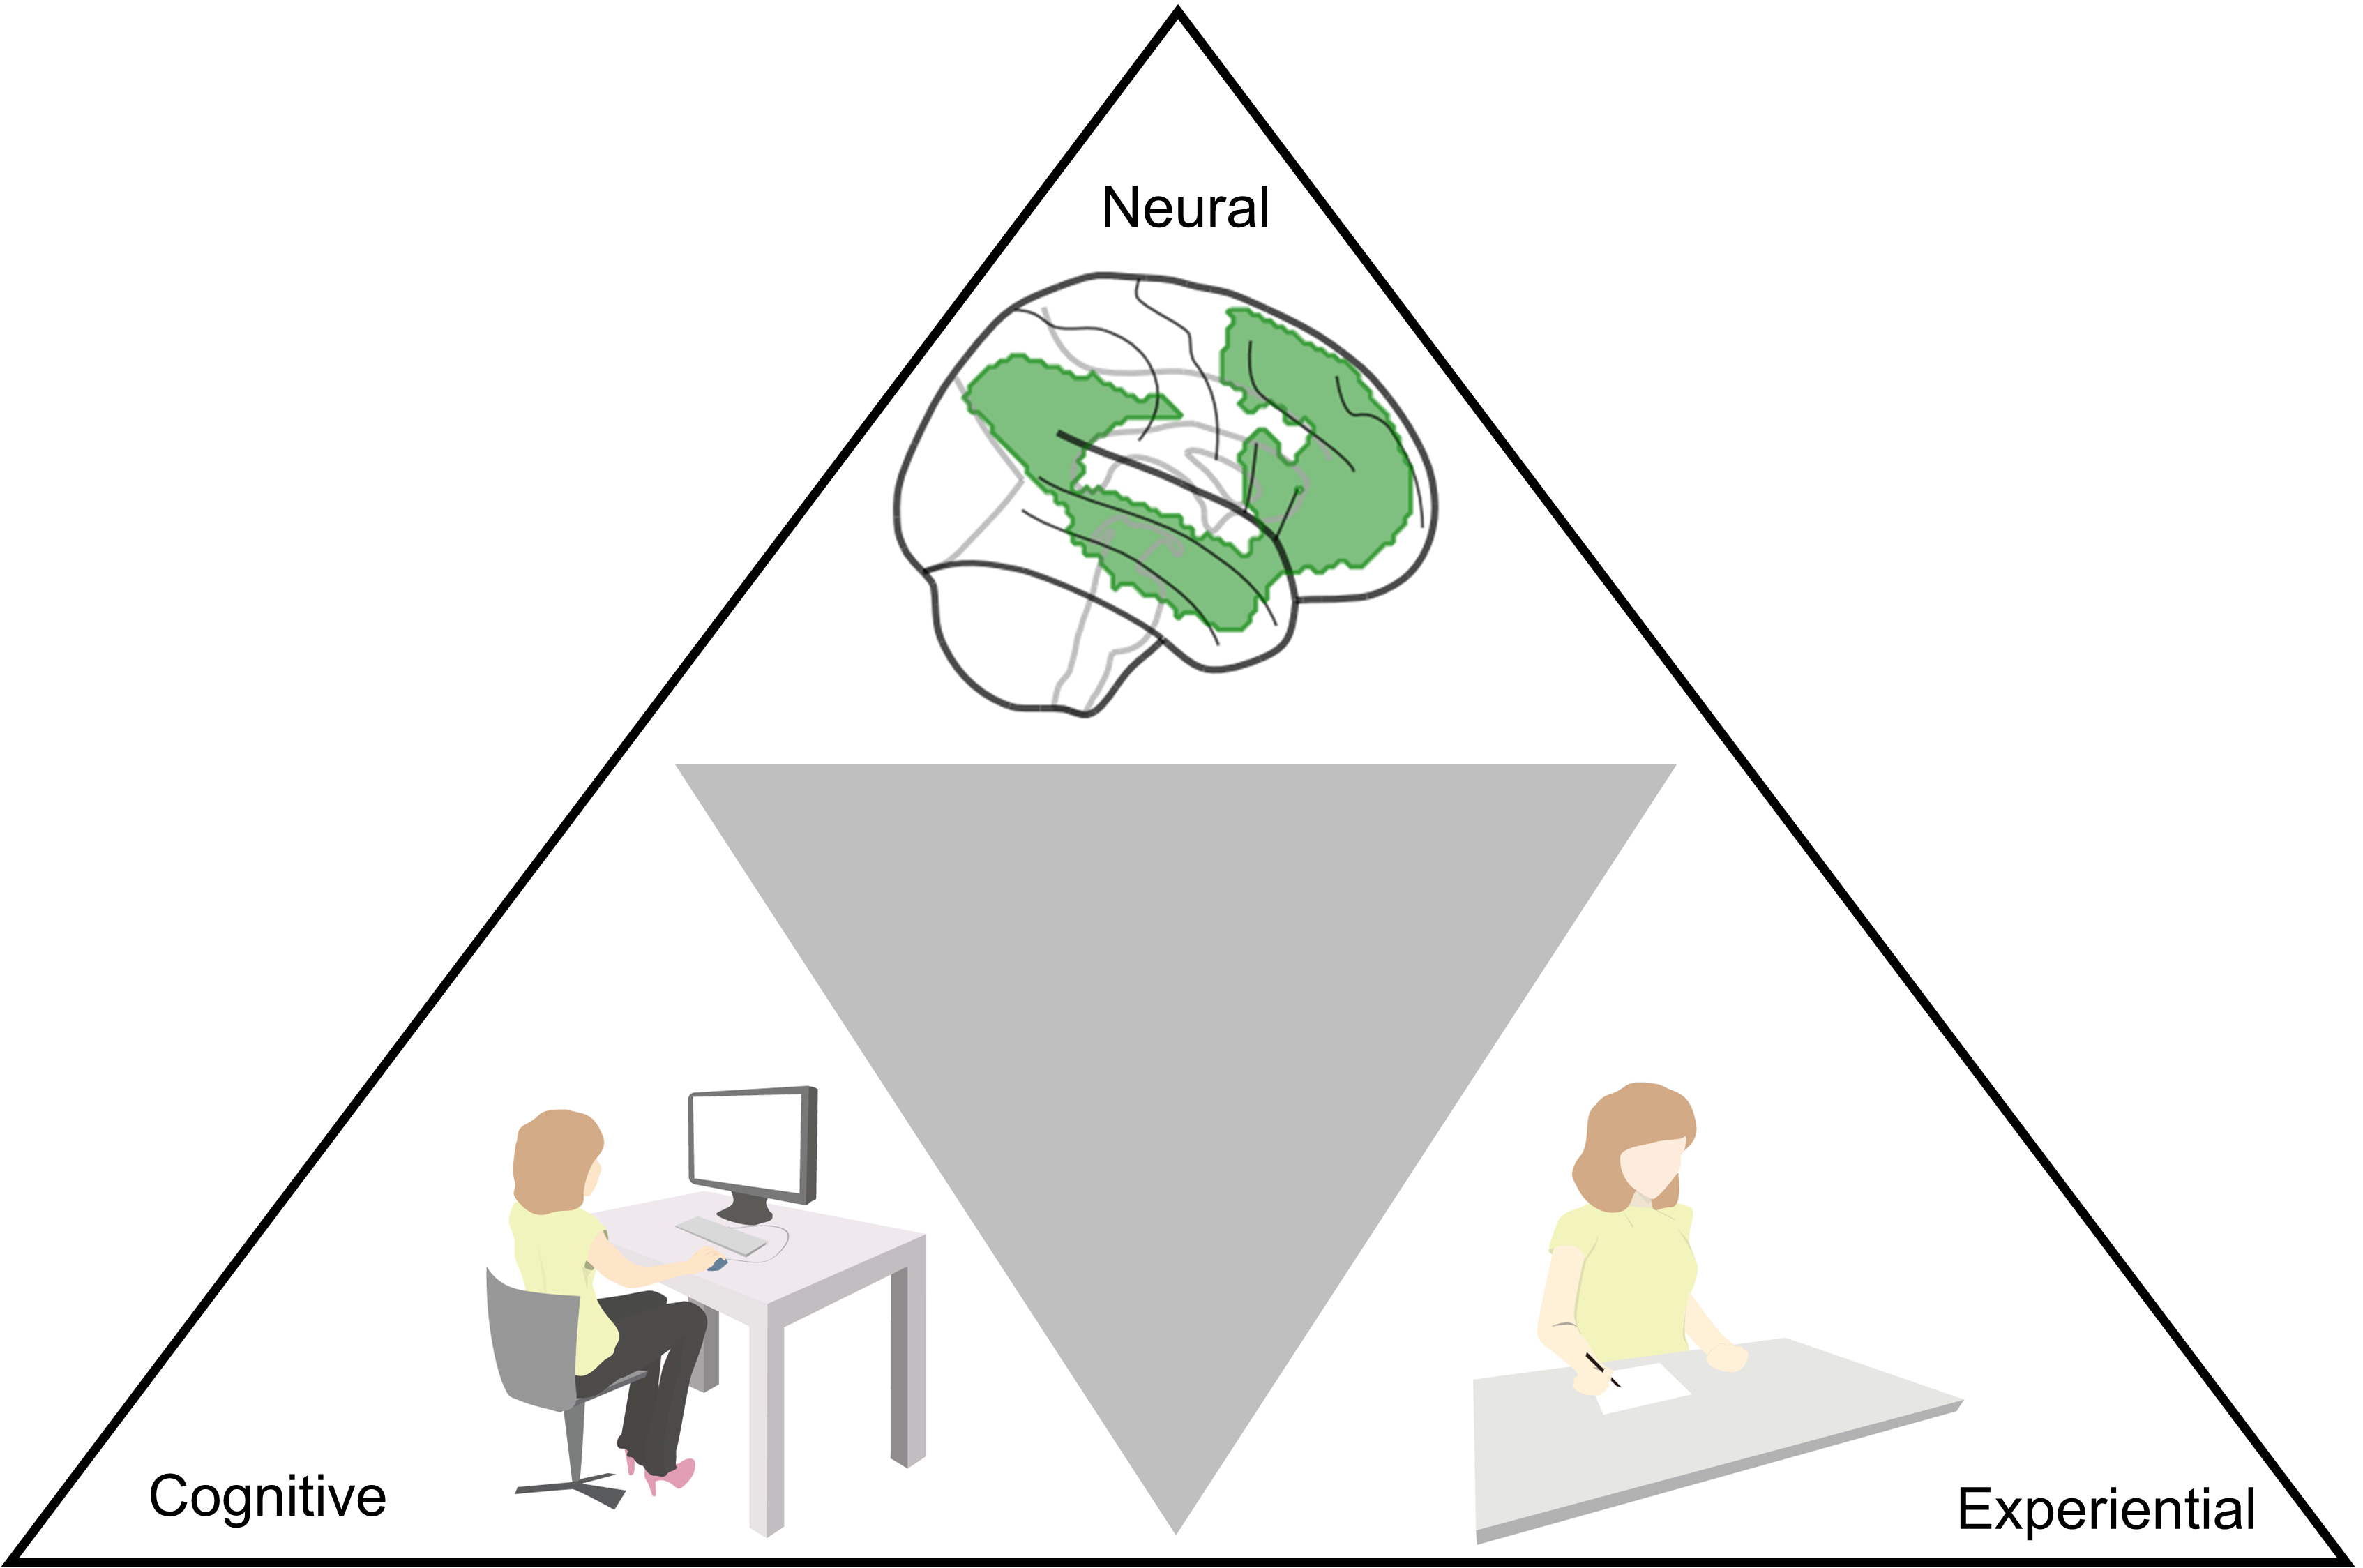
\includegraphics[width=0.8\textwidth]{chapters/img/thesisfig1.png}
	\caption{Schematic of the thesis} 
	\label{fig:thesis:fig1}
\end{figure}

% ==========================================================================================================
\section{Mind wandering measuring methods and current progress}
\label{intro:measures}

\subsection{Content of experience}

\subsection{Method of acquiring experience}
Mind-wandering can be measured in both online and retrospective manners, and the two methods have different advantages for describing the mind-wandering state (Smallwood \& Schooler, 2015). Experience sampling reports the momentary, natural evolution of thoughts. By random probing during a given task, this technique measures the change in thoughts under different time course. The disadvantage is that the probe interrupts the task or the ongoing thoughts, therefore it could be seen as an extra task that alternates the nature of the mind-wandering state. Off-line report is a retrospective report on the summary of the mind-wandering experience after the task. The benefit of this method is that there are no interruption during the given task or the on-going thoughts, but its reliability on demonstrating the natural train 0f thoughts is in question.  Despites these methods describe two distinct aspect of mind wandering, studies reveal similar properties for both online and retrospective measures for both attention and happiness. Kam and colleagues (Kam et al., 2012) demonstrates that experience sampling reports the momentary change in attention, using experience sampling along with event-related potential (ERP) as a measurement of attention. Off-line report is also a reliable measure, proofed by the correlation between the report and their ERP measures on attention in task (Barron, Riby, Greer, \& Smallwood, 2011). The similarity of these two technique has been demonstrated by Smallwood and O'Connor’s study on happiness, where an unhappy mood revealed by the online experience sampling increases past thinking in the retrospective report off-line (Smallwood \& O’Connor, 2011). Perhaps the similarity between the off-line report and experience sampling indicates that spontaneous thought has a consistent pattern in the mind-wandering states across different situations. 

Previous studies have identified various features related to cognitive function. To access the complex, heterogeneous content of spontaneous thoughts, researchers have employed Mulit-Dimension Experience Sampling (MDES; Medea et al., 2016; Ruby, Smallwood, Engen, et al., 2013; Smallwood et al., 2016) method. MDES quantifies the momentary experience related to a wide range of form and content of thoughts. Measuring multiple dimensions facilitated the heterogeneity hypothesis of the mind-wandering state. The questions in MDES are can be used not just in an on-going cognitive task, but also collect the retrospective, off-line report to understand the general state-like feature of the mind-wandering experience. 


\subsection{Method of describing the neural organisation using CCA}
% ==========================================================================================================
\section{Summary}

% ==========================================================================================================
